\ifdefined\gkver\else\def\gkver{student}\fi
\documentclass[\gkver]{gaokaozhenti}
\begin{document}

\chapter{2025年6月浙江}

\begin{enumerate}
\item
%% number: 1
%% paperName: 2025年6月浙江高考第 1 题 3 分
%% typeId: 1
%% type: 单选题
%% chapter: 运动和力
%% point: 力学单位制
%% method: 无
%% score: 3
%% degree: 950
%% duplicateId: 0
%% body:
光子能量 $E = h\nu$，式中 $\nu$ 是光子的频率，$h$ 是普朗克常量。$h$ 的单位是\xzanswer{A}

\fourchoices[answer=A]
{$\UJcdots[a]$}
{$\UNs[a]$}
{$\Ukg[a]$}
{$\Um[a]$}

%% answer: A
%% memo:
\memoanswer{
根据公式 $E = h\nu$，能量 $E$ 的单位是焦耳（J），频率 $\nu$ 的单位是赫兹（Hz，即 $\Usn$）。

因此，普朗克常量 $h$ 的单位为 $h = \frac{E}{\nu} = \frac{\UJ}{\Usn} = \UJcdots$。

故选 A。
}

\item
%% number: 2
%% paperName: 2025年6月浙江高考第 2 题 3 分
%% typeId: 1
%% type: 单选题
%% chapter: 直线运动
%% point: 质点
%% method: 无
%% score: 3
%% degree: 750
%% duplicateId: 0
%% body:
2025 年 4 月 30 日，“神舟十九号载人飞船”返回舱安全着陆，宇航员顺利出舱。在其返回过程中，下列说法正确的是\xzanswer{A}

\fourchoices[answer=A]
{研究返回舱运行轨迹时，可将其视为质点}
{随着返回舱不断靠近地面，地球对其引力逐渐减小}
{返回舱落地前，反推发动机点火减速，宇航员处于失重状态}
{用返回舱的轨迹长度和返回时间，可计算其平均速度的大小}

%% answer: A
%% memo:
\memoanswer{
A．当物体的大小和形状对所研究的问题影响可忽略时可将其视为质点，研究返回舱的运行轨迹时，其尺寸远小于轨迹长度，形状和结构不影响轨迹分析，可将其视为质点，故 A 正确；

B．地球对返回舱的引力由公式 $F = \frac{GMm}{r^{2}}$ 决定，其中 $r$ 为返回舱到地心的距离，返回舱靠近地面时，$r$ 减小，引力增大，故 B 错误；

C．反推发动机点火减速时，返回舱的加速度方向向上。根据牛顿第二定律，宇航员受到的支持力大于重力，处于超重状态，而非失重状态，故 C 错误；

D．平均速度的定义是位移与时间的比值，而轨迹长度为路程，轨迹长度与时间的比值是平均速率，而非平均速度的大小，故 D 错误。

故选 A。
}

\item
%% number: 3
%% paperName: 2025年6月浙江高考第 3 题 3 分
%% typeId: 1
%% type: 单选题
%% chapter: 曲线运动
%% point: 平抛运动
%% method: 无
%% score: 3
%% degree: 650
%% duplicateId: 0
%% body:
如图所示，在水平桌面上放置一斜面，在桌边水平放置一块高度可调的木板。让钢球从斜面上同一位置静止滚下，越过桌边后做平抛运动。当木板离桌面的竖直距离为 $h$ 时，钢球在木板上的落点离桌边的水平距离为 $x$，则\xzanswer{B}

\onepicture[w=5.4cm]{figs/03.png}

\fourchoices[answer=B]
{钢球平抛初速度为 $x\sqrt{\frac{2h}{g}}$}
{钢球在空中飞行时间为 $\sqrt{\frac{2h}{g}}$}
{增大 $h$，钢球撞击木板的速度方向不变}
{减小 $h$，钢球落点离桌边的水平距离不变}

%% answer: B
%% memo:
\memoanswer{
AB．根据平抛运动的规律可知，钢球在空中飞行时间为 $t = \sqrt{\frac{2h}{g}}$

钢球平抛初速度为 $v_{0} = \frac{x}{t} = x\sqrt{\frac{g}{2h}}$，A 错误，B 正确；

C．钢球撞击木板时速度方向与水平方向的夹角满足 $\tan\theta = \frac{v_{y}}{v_{0}} = \frac{\sqrt{2gh}}{v_{0}}$

可知，增大 $h$，钢球撞击木板的速度方向与水平方向的夹角变大，C 错误；

D．根据 $x = v_{0}\sqrt{\frac{2h}{g}}$ 可知，减小 $h$，钢球落点离桌边的水平距离 $x$ 减小，D 错误。

故选 B。
}

\item
%% number: 4
%% paperName: 2025年6月浙江高考第 4 题 3 分
%% typeId: 1
%% type: 单选题
%% chapter: 光学
%% point: 波粒二象性
%% method: 无
%% score: 3
%% degree: 750
%% duplicateId: 0
%% body:
一束高能电子穿过铝箔，在铝箔后方的屏幕上观测到如图所示的电子衍射图样，则\xzanswer{C}

\onepicture[w=3.6cm]{figs/04.jpg}

\fourchoices[answer=C]
{该实验表明电子具有粒子性}
{图中亮纹为电子运动的轨迹}
{图中亮纹处电子出现的概率大}
{电子速度越大，中心亮斑半径越大}

%% answer: C
%% memo:
\memoanswer{
A．该实验表明电子具有波动性，A 错误；

BC．根据“概率波”特点可知，图中亮纹处电子出现的概率大，亮纹处并非电子运动的轨迹，B 错误，C 正确；

D．根据物质波的表达式有 $\lambda = \frac{h}{p} = \frac{h}{mv}$

可知，电子的速度越大，其物质波波长变短，衍射现象越不明显，则中心亮斑半径越小，D 错误。

故选 C。
}

\item
%% number: 5
%% paperName: 2025年6月浙江高考第 5 题 3 分
%% typeId: 1
%% type: 单选题
%% chapter: 交流电
%% point: LC振荡回路
%% method: 无
%% score: 3
%% degree: 750
%% duplicateId: 0
%% body:
如图所示的 $LC$ 振荡电路，能减小其电磁振荡周期的措施是\xzanswer{D}

\onepicture[w=2.6cm]{figs/05.png}

\fourchoices[answer=D, ispicture=true, h=2.20cm]
{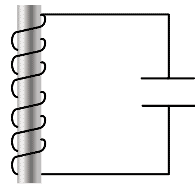
\includegraphics{figs/05a.png}\\线圈中插入铁芯}
{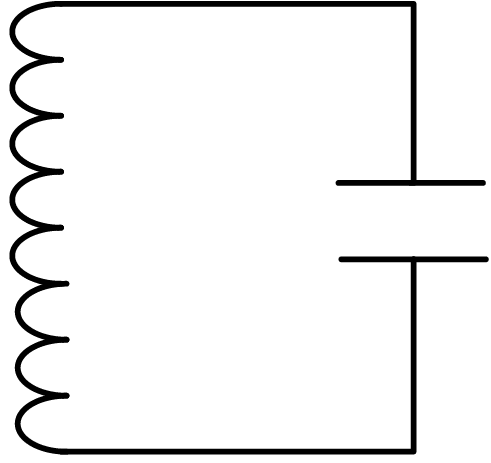
\includegraphics{figs/05b.png}\\线圈匝数增加}
{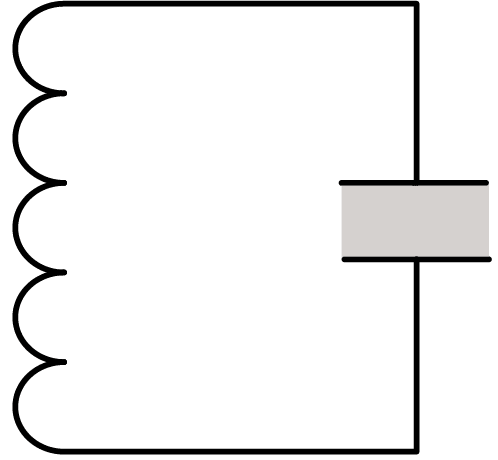
\includegraphics{figs/05c.png}\\电容器极板间插入电介质}
{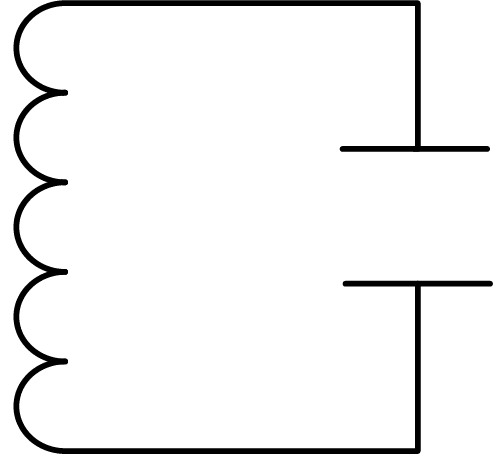
\includegraphics{figs/05d.png}\\电容器极板间距增大}

%% answer: D
%% memo:
\memoanswer{
A．线圈中插入铁芯，增大了自感系数 $L$，由电磁振荡的周期 $T = 2\pi\sqrt{LC}$ 可知周期变大，故 A 错误；

B．线圈的匝数增多，自感系数 $L$ 变大，由 $T = 2\pi\sqrt{LC}$ 可知周期变大，故 B 错误；

C．电容器极板间插入电介质，即增大 $\varepsilon_{r}$，由 $C = \frac{\varepsilon_{r}S}{4\pi kd}$ 可知电容变大，由 $T = 2\pi\sqrt{LC}$ 可知周期变大，故 C 错误；

D．电容器极板间距 $d$ 增大，由 $C = \frac{\varepsilon_{r}S}{4\pi kd}$ 可知电容变小，由 $T = 2\pi\sqrt{LC}$ 可知周期变小，故 D 正确。

故选 D。
}

\item
%% number: 6
%% paperName: 2025年6月浙江高考第 6 题 3 分
%% typeId: 1
%% type: 单选题
%% chapter: 功和能
%% point: 动能定理
%% method: 无
%% score: 3
%% degree: 550
%% duplicateId: 0
%% body:
如图所示，两根相同的橡皮绳，一端连接质量为 $m$ 的物块，另一端固定在水平桌面上的 A、B 两点。物块处于 AB 连线的中点 C 时，橡皮绳为原长。现将物块沿 AB 中垂线水平拉至桌面上的 O 点静止释放。已知 CO 距离为 $L$，物块与桌面间的动摩擦因数为 $\mu$，橡皮绳始终处于弹性限度内，不计空气阻力，则释放后\xzanswer{D}

\onepicture[w=4.4cm]{figs/06.png}

\fourchoices[answer=D]
{物块做简谐运动}
{物块只受到重力、橡皮绳弹力和摩擦力的作用}
{若 $\angle AOB = 90^{\circ}$ 时每根橡皮绳的弹力为 $F$，则物块所受合力大小为 $\sqrt{2}F$}
{若物块第一次到达 C 点的速度为 $v_{0}$，此过程中橡皮绳对物块做的功 $W = \frac{1}{2}mv_{0}^{2} + \mu mgL$}

%% answer: D
%% memo:
\memoanswer{
AB．物块在水平桌面上运动，受到重力、桌面的支持力、橡皮绳的弹力以及摩擦力的作用；而运动方向受橡皮绳的弹力和摩擦力作用，其合力不满足简谐运动的回复力特点（$F = -kx$），因摩擦力是恒力，不随位移按比例变化，所以物块不做简谐运动，故 AB 错误；

C．若 $\angle AOB = 90^{\circ}$ 时每根橡皮绳的弹力为 $F$，两根橡皮绳弹力的合力 $F_{\text{弹合}} = \sqrt{F^{2} + F^{2}} = \sqrt{2}F$

物块还受到摩擦力为 $f = \mu N = \mu mg$

则物块所受合力为 $F_{\text{合}} = \sqrt{2}F - \mu mg$，故 C 错误；

D．若物块第一次到达 C 点的速度为 $v_{0}$，物块从 O 点运动到 C 点，由动能定理可知 $W - \mu mgL = \frac{1}{2}mv_{0}^{2} - 0$

解得橡皮绳对物块做的功为 $W = \frac{1}{2}mv_{0}^{2} + \mu mgL$，故 D 正确。

故选 D。
}

\item
%% number: 7
%% paperName: 2025年6月浙江高考第 7 题 3 分
%% typeId: 1
%% type: 单选题
%% chapter: 电路
%% point: 电功电功率
%% method: 无
%% score: 3
%% degree: 550
%% duplicateId: 0
%% body:
如图所示，风光互补环保路灯的主要构件有：风力发电机，单晶硅太阳能板，额定电压 $48\UV$、容量 $200\UAh$ 的储能电池，功率 $60\UW$ 的 LED 灯。已知该路灯平均每天照明 $10\Uh$；$1\Ukg$ 标准煤完全燃烧可发电 2.8 度，排放二氧化碳 $2.6\Ukg$。则\xzanswer{D}

\onepicture[w=4.6cm]{figs/07.jpg}

\fourchoices[answer=D]
{风力发电机的输出功率与风速的平方成正比}
{太阳能板上接收到的辐射能全部转换成电能}
{该路灯正常运行 6 年，可减少二氧化碳排放量约 $1.2 \times 10^{6}\Ukg$}
{储能电池充满电后，即使连续一周无风且阴雨，路灯也能正常工作}

%% answer: D
%% memo:
\memoanswer{
A．设 $\Delta t$ 时间，风力发电机的扇叶半径为 $r$，假设风的动能全部变成发电机输出，输出功率为 $P_{\text{出}} = \frac{\frac{1}{2}mv^{2}}{\Delta t} = \frac{\frac{1}{2}\rho \cdot \pi r^{2} \cdot v \cdot \Delta t \cdot v^{2}}{\Delta t} = \frac{1}{2}\rho\pi r^{2}v^{3}$，即风力发电机的输出功率与风速的三次方成正比，故 A 错误；

B．太阳能板上接收到的辐射能不能全部转换成电能，存在能量损耗，转换效率一般在 15%～20% 左右，故 B 错误；

C．已知路灯的功率为 $P = 60\UW = 0.06\UkW$

每天照明 $t = 10\Uh$，一年按 365 天计算，6 年的总时间 $t_{\text{总}} = 6 \times 365 \times 10\Uh = 21900\Uh$

可得总耗电量为 $W = Pt_{\text{总}} = 0.06\UkW \times 21900\Uh = 1314\UkWh = 1314$ 度

因 $1\Ukg$ 标准煤完全燃烧可发电 2.8 度，排放二氧化碳 $2.6\Ukg$，则减少的二氧化碳排放量为 $M = \frac{1314}{2.8} \times 2.6\Ukg \approx 1230\Ukg \neq 1.2 \times 10^{6}\Ukg$，故 C 错误；

D．已知储能电池的额定电压 $U = 48\UV$，容量 $Q = 200\UAh$，则电池的电能为 $E = UQ = 9600\UWh = 9.6\UkWh$

而路灯连续一周的耗电量为 $W = Pt = 0.06\UkW \times 7 \times 10\Uh = 4.2\UkWh$

因 $9.6\UkWh > 4.2\UkWh$，所以储能电池充满电后，即使连续一周无风且阴雨，路灯也能正常工作。故 D 正确。

故选 D。
}

\item
%% number: 8
%% paperName: 2025年6月浙江高考第 8 题 3 分
%% typeId: 1
%% type: 单选题
%% chapter: 电场
%% point: 带电粒子的轨迹类问题
%% method: 无
%% score: 3
%% degree: 650
%% duplicateId: 0
%% body:
一束 $\alpha$ 粒子撞击一静止的金原子核，它们的运动轨迹如图所示。图中虚线是以金原子核为圆心的圆。已知静电力常量 $k = 9.0 \times 10^{9}\UNmqCq$，元电荷 $e = 1.6 \times 10^{-19}\UC$，金原子序数为 79，不考虑 $\alpha$ 粒子间的相互作用，则\xzanswer{D}

\onepicture[w=5.3cm]{figs/08.png}

\fourchoices[answer=D]
{沿轨迹 1 运动的 $\alpha$ 粒子受到的库仑力先做正功，后做负功}
{沿轨迹 2 运动的 $\alpha$ 粒子到达 P 时动能为零、电势能最大}
{位于图中虚线圆周上的 3 个 $\alpha$ 粒子的电势能不相等}
{若 $\alpha$ 粒子与金原子核距离为 $10^{-14}\Um$，则库仑力数量级为 $10^{2}\UN$}

%% answer: D
%% memo:
\memoanswer{
A．沿轨迹 1 运动的 $\alpha$ 粒子受到的库仑力先做负功，后做正功，A 错误；

B．沿轨迹 2 运动的 $\alpha$ 粒子因为做曲线运动，则到达 P 时动能不为零，因距离原子核最近，则电势能最大，B 错误；

C．位于图中虚线圆周上各点的电势都相等，可知虚线圆周上的 3 个 $\alpha$ 粒子的电势能相等，C 错误；

D．若 $\alpha$ 粒子与金原子核距离为 $10^{-14}\Um$，则根据库仑定律可知库仑力 $F = k\frac{qQ}{r^{2}} = 9 \times 10^{9} \times \frac{2 \times 1.6 \times 10^{-19} \times 79 \times 1.6 \times 10^{-19}}{(10^{-14})^{2}}\UN = 364\UN$

即数量级为 $10^{2}\UN$，D 正确。

故选 D。
}

\item
%% number: 9
%% paperName: 2025年6月浙江高考第 9 题 3 分
%% typeId: 1
%% type: 单选题
%% chapter: 功和能
%% point: 动能定理
%% method: 近似与估算
%% score: 3
%% degree: 550
%% duplicateId: 0
%% body:
高空抛物伤人事件时有发生，成年人头部受到 $500\UN$ 的冲击力，就会有生命危险。设有一质量为 $50\Ug$ 的鸡蛋从高楼坠落，以鸡蛋上、下沿接触地面的时间差作为其撞击地面的时间，上、下沿距离为 $5\Ucm$，要产生 $500\UN$ 的冲击力，估算鸡蛋坠落的楼层为\xzanswer{C}

\fourchoices[answer=C]
{5 层}
{8 层}
{17 层}
{27 层}

%% answer: C
%% memo:
\memoanswer{
鸡蛋触地后匀减速至静止，位移 $s = 5\Ucm = 0.05\Um$。匀减速平均速度为 $\frac{v}{2}$，故撞击时间 $\Delta t = \frac{2s}{v}$

根据动量定理 $(F - mg)\Delta t = 0 - (-mv)$

代入数据解得 $v \approx \sqrt{1000}\Ums$

由自由落体公式 $v^{2} = 2gh$

得高度 $h = \frac{v^{2}}{2g} = \frac{1000}{2 \times 9.8}\Um \approx 51\Um$

每层楼高约 $3\Um$，对应楼层数为 $\frac{51}{3} = 17$ 层。

故选 C。
}

\item
%% number: 10
%% paperName: 2025年6月浙江高考第 10 题 3 分
%% typeId: 1
%% type: 单选题
%% chapter: 交流电
%% point: 交流电
%% method: 无
%% score: 3
%% degree: 450
%% duplicateId: 0
%% body:
如图甲所示，有一根长 $1\Um$、两端固定紧绷的金属丝，通过导线连接示波器。在金属丝中点处放置一蹄形磁铁，在中点附近 $1.00\Ucm$ 范围内产生 $B = 10^{-3}\UT$、方向垂直金属丝的匀强磁场（其他区域磁场忽略不计）。现用一激振器使金属丝发生垂直于磁场方向的上下振动，稳定后形成如图乙所示的不同时刻的波形，其中最大振幅 $A = 0.5\Ucm$。若振动频率为 $f$，则振动最大速度 $v = 2\pi fA$。已知金属丝接入电路的电阻 $r = 0.5\UO$，示波器显示输入信号的频率为 $150\UHz$。下列说法正确的是\xzanswer{C}

\onepicture[w=11.0cm]{figs/10.png}

\fourchoices[answer=C]
{金属丝上波的传播速度为 $\frac{3}{2}\pi\Ums$}
{金属丝产生的感应电动势最大值约为 $\frac{3}{2}\pi \times 10^{-3}\UV$}
{若将示波器换成可变电阻，则金属丝的最大输出功率约为 $\frac{9}{16}\pi^{2} \times 10^{-10}\UW$}
{若让激振器产生沿金属丝方向的振动，其他条件不变，则金属丝中点的振幅为零}

%% answer: C
%% memo:
\memoanswer{
A．先由图可判断金属丝振动形成三节（如图乙所示共有三个波腹），则波长为 $\lambda = \frac{2}{3}L = \frac{2}{3}\Um$

又振动频率为 $f = 150\UHz$，可得波速为 $v = \lambda f = 100\Ums$，故 A 错误；

B．金属丝在中点附近的匀强磁场中振动，其振动最大速度为 $v_{m} = 2\pi fA$

其中 $A = 0.5\Ucm = 0.005\Um$，$f = 150\UHz$，计算得 $v_{m} = 2\pi \times 150 \times 0.005\Ums = 1.5\pi\Ums$

中点切割的有效长度为 $L = 0.01\Um$

则中点处感应电动势最大值为 $E_{\text{max}} = BLv_{m} = \frac{3}{2}\pi \times 10^{-5}\UV$，故 B 错误；

C．金属丝在中点附近的匀强磁场中振动，产生的是正弦式交流电，电动势的有效值为 $E = \frac{E_{\text{max}}}{\sqrt{2}}$，若用最大感应电动势 $E_{\text{max}} = \frac{3}{2}\pi \times 10^{-5}\UV$ 接外电阻，则金属丝本身内阻 $r = 0.5\UO$，正弦交流源在内阻 $r$ 和外阻 $R$ 串联时，当 $R = r = 0.5\UO$ 时可得最大输出功率为 $P_{\text{max}} = \frac{(\frac{E_{\text{max}}}{\sqrt{2}})^{2}}{4r} = \frac{9}{16}\pi^{2} \times 10^{-10}\UW$，故 C 正确；

D．若改为沿金属丝方向振动形成纵波，两端固定则端点处必为纵波的振动节（位移为零处），其基频振型中点恰为振幅最大处（波腹），并非振幅为零，故 D 错误。

故选 C。
}

\item
%% number: 11
%% paperName: 2025年6月浙江高考第 11 题 4 分
%% typeId: 2
%% type: 多选题
%% chapter: 交流电
%% point: 变压器
%% method: 无
%% score: 4
%% degree: 650
%% duplicateId: 0
%% body:
下列说法正确的是\xzanswer{CD}

\fourchoices[answer=CD]
{热量能自发地从低温物体传到高温物体}
{按照相对论的时间延缓效应，低速运动的微观粒子寿命比高速运动时更长}
{变压器原线圈中电流产生的变化磁场，在副线圈中激发感生电场，从而产生电动势}
{热敏电阻和电阻应变片两种传感器，都是通过测量电阻，确定与之相关的非电学量}

%% answer: CD
%% memo:
\memoanswer{
A．根据热力学第二定律可知热量不能自发地从低温物体传到高温物体，故 A 错误；

B．按照相对论的时间延缓效应，运动的时钟会变慢。对于微观粒子，高速运动时其内部的时间进程变慢，相当于寿命变长；而低速运动时，时间延缓效应不明显，其寿命比高速运动时更短，故 B 错误；

C．变压器的工作原理是电磁感应。原线圈中电流产生的变化磁场，穿过副线圈时，会在副线圈中激发感生电场，感生电场对副线圈中的自由电荷有作用力，从而产生电动势，这就是变压器副线圈产生感应电动势的原理，故 C 正确；

D．电阻传感器是通过测量电阻的变化来确定与之相关的非电学量，比如温度传感器，温度变化会引起电阻变化，通过测量电阻就可以知道温度的变化。电阻应变片是基于电阻应变效应工作的，当应变片受到外力作用发生形变时，其电阻值会发生变化，通过测量电阻变化可以确定外力等非电学量，故 D 正确。

故选 CD。
}

\item
%% number: 12
%% paperName: 2025年6月浙江高考第 12 题 4 分
%% typeId: 2
%% type: 多选题
%% chapter: 原子和原子核
%% point: 玻尔模型
%% method: 无
%% score: 4
%% degree: 550
%% duplicateId: 0
%% body:
氢原子从 $n = 4$、6 的能级向 $n = 2$ 的能级跃迁时分别发出光 P、Q。则\xzanswer{BC}

\onepicture[w=14.0cm]{figs/12.png}

\fourchoices[answer=BC]
{P、Q 经过甲图装置时屏上谱线分别为 2、1}
{若乙图玻璃棒能导出 P 光，则一定也能导出 Q 光}
{若丙图是 P 入射时的干涉条纹，则 Q 入射时条纹间距减小}
{P、Q 照射某金属发生光电效应，丁图中的点 1、2 分别对应 P、Q}

%% answer: BC
%% memo:
\memoanswer{
A．氢原子从 $n = 4$、6 的能级向 $n = 2$ 的能级跃迁时分别发出光 P、Q。则 P 光对应的光子能量较小，光子的频率较小，P 光的折射率较小，则经过甲图装置时 P 光的偏折程度较小，则 P、Q 在屏上谱线分别为 1、2，A 错误；

B．根据 $\sin C = \frac{1}{n}$ 可知，P 光折射率较小，则发生全反射的临界角较大，若乙图玻璃棒能导出 P 光，则一定也能导出 Q 光，B 正确；

C．若丙图是 P 入射时的干涉条纹，因 P 光波长大于 Q 光，则 Q 入射时条纹间距减小，C 正确；

D．根据 $E_{k} = h\nu - W_{\text{逸出功}}$ 可知因 P 光频率小于 Q 光，可知丁图中的点 1、2 分别对应 Q、P 光，D 错误。

故选 BC。
}

\item
%% number: 13
%% paperName: 2025年6月浙江高考第 13 题 4 分
%% typeId: 2
%% type: 多选题
%% chapter: 曲线运动
%% point: 开普勒定律
%% method: 无
%% score: 4
%% degree: 350
%% duplicateId: 0
%% body:
月球有类似于地球的南北两极和纬度。如图所示，月球半径为 $R$，表面重力加速度为 $g_{\text{月}}$，不考虑月球自转。从月球北极正上方水平发射一物体，要求落在纬度 $\varphi = 60^{\circ}$ 的 M 处，其运动轨迹为椭圆的一部分。假设月球质量集中在球心 O 点，如果物体沿椭圆运动的周期最短，则\xzanswer{BC}

\onepicture[h=5.0cm, align=right]{figs/13.png}

\fourchoices[answer=BC]
{发射点离月面的高度 $h = \frac{\sqrt{3}}{4}R$}
{物体沿椭圆运动的周期为 $\frac{3\pi}{4}\sqrt{\frac{3R}{g_{\text{月}}}}$}
{此椭圆两焦点之间的距离为 $\frac{\sqrt{3}}{2}R$}
{若水平发射的速度为 $v$，发射高度为 $h$，则物体落到 M 处的速度 $\sqrt{v^{2} + 2g_{\text{月}}h}$}

%% answer: BC
%% memo:
\memoanswer{
根据题意可知椭圆轨道的一个焦点为 O，设椭圆的另外一个焦点为 $O'$，如图所示。

\onepicture[h=4.0cm]{figs/13_an1.png}

设椭圆的半长轴为 $a$，焦距为 $2c$，根据椭圆知识可知 $O'M + OM = 2a$

根据开普勒第三定律 $\frac{a^{3}}{T^{2}} = C$ 可知如果物体沿椭圆运动的周期最短，则椭圆的半长轴最小，根据几何关系可知当 $MO'$ 垂直于 $OO'$ 时，半长轴 $a$ 最小，如图所示。

\onepicture[h=4.0cm]{figs/13_an2.png}

由几何关系有 $2a = R\cos\varphi + R$

解得 $a = \frac{3R}{4}$

C．根据几何关系可得椭圆的焦距 $2c = OO' = R\sin\varphi = \frac{\sqrt{3}R}{2}$，故 C 正确；

A．根据几何关系可得发射点离月面的高度 $h = a + c - R = \frac{\sqrt{3} - 1}{4}R$，故 A 错误；

B．设物体绕月球表面做匀速圆周运动时的周期为 $T_{0}$，则由重力提供向心力得 $mg_{\text{月}} = m\frac{4\pi^{2}}{T_{0}^{2}}R$

结合开普勒第三定律 $\frac{R^{3}}{T_{0}^{2}} = \frac{a^{3}}{T^{2}}$

联立可得物体沿椭圆运动的周期为 $T = \frac{3\pi}{4}\sqrt{\frac{3R}{g_{\text{月}}}}$，故 B 正确；

D．由引力势能公式 $E_{p} = -\frac{GMm}{r}$

结合万有引力公式 $m'g_{\text{月}} = G\frac{Mm'}{R^{2}}$

结合机械能守恒定律有 $-\frac{GMm'}{R + h} + \frac{1}{2}m'v^{2} = -\frac{GMm'}{R} + \frac{1}{2}m'v_{M}^{2}$

联立可得 $v_{M} = \sqrt{v^{2} + \frac{2g_{\text{月}}hR}{R + h}}$，故 D 错误。

故选 BC。
}

\item
%% number: 14
%% paperName: 2025年6月浙江高考第 14 题 7 分
%% typeId: 4
%% type: 实验题
%% chapter: 机械振动
%% point: 单摆测重力加速度
%% method: 无
%% score: 7
%% degree: 450
%% duplicateId: 0
%% body:
（一）在测量一节干电池的电动势和内阻的实验中。

\onepicture[h=2.60cm, align=right]{figs/14a.png}

\begin{enumerate}
	\item
	为了减小测量误差，如图所示的电路中应该选择的是\tkanswer{甲}（选填“甲”或“乙”）；
	\item
	通过调节滑动变阻器，测得多组 $U$、$I$ 数据，记录于下表。试在\textbf{答题纸}上的方格纸中建立合适的标度，描点并作出 $U-I$ 图像，由此求得电动势 $E =$\tkanswer{1.46 \textasciitilde{} 1.48}$\UV$，内阻 $r =$\tkanswer{0.61 \textasciitilde{} 0.63}$\UO$。（结果均保留到小数点后两位）
\end{enumerate}

\begin{center}
\small
\begin{tabular}{|c|c|c|c|c|c|}
\hline
次数 & 1 & 2 & 3 & 4 & 5 \\
\hline
$U/\UV$ & 1.35 & 1.30 & 1.25 & 1.20 & 1.15 \\
\hline
$I/\UA$ & 0.14 & 0.22 & 0.30 & 0.37 & 0.45 \\
\hline
\end{tabular}
\end{center}

（二）在用单摆测重力加速度的实验中。

\onepicture[h=2.80cm, align=right]{figs/14b.png}

\begin{enumerate}
	\item
	如图 1 所示，可在单摆悬点处安装力传感器，也可在摆球的平衡位置处安装光电门。甲同学利用力传感器，获得传感器读取的力与时间的关系图像，如图 2 所示，则单摆的周期为\tkanswer{1.31}$\Us$（结果保留 3 位有效数字）。乙同学利用光电门，从小钢球第 1 次遮光开始计时，记下第 $n$ 次遮光的时刻 $t$，则单摆的周期为 $T =$\tkanswer{$\frac{2t}{n - 1}$}；
	\item
	丙同学发现小钢球已变形，为减小测量误差，他改变摆线长度 $l$，测出对应的周期 $T$，作出相应的 $l-T^{2}$ 关系图线，如图 3 所示。由此算出图线的斜率 $k$ 和截距 $b$，则重力加速度 $g =$\tkanswer{$\frac{4\pi^{2}}{k}$}，小钢球重心到摆线下端的高度差 $h =$\tkanswer{$kb$}；（结果均用 $k$、$b$ 表示）
	\item
	丁同学用 3D 打印技术制作了一个圆心角等于 $5^{\circ}$、半径已知的圆弧槽，如图 4 所示。他让小钢球在槽中运动，测出其运动周期，算出重力加速度为 $8.64\Umsq$。若周期测量无误，则获得的重力加速度明显偏离实际值的最主要原因是\tkanswer{小钢球有具体形状和大小，不能将其看作质点，其质心的运动轨迹半径与圆弧槽半径有偏差，导致计算时所用“摆长”不准确}。
\end{enumerate}

%% answer:
\jdanswer{
\begin{enumerate}
	\item
	甲
	\item
	$1.46 \sim 1.48$，$0.61 \sim 0.63$
\end{enumerate}
\begin{enumerate}
	\item
	$1.31$，$\frac{2t}{n - 1}$
	\item
	$\frac{4\pi^{2}}{k}$，$kb$
	\item
	小钢球有具体形状和大小，不能将其看作质点，其质心的运动轨迹半径与圆弧槽半径有偏差，导致计算时所用“摆长”不准确。
\end{enumerate}
}
%% memo:
\memoanswer{
（一）（1）因乙电路中电流表内阻对电源内阻的测量影响较大，则为了减小测量误差，如图所示的电路中应该选择的是甲；

（2）根据实验数据做出电源的 $U-I$ 图像如图

\onepicture[h=5.00cm]{figs/14a_an.png}

由 $U = E - Ir$ 结合图像可知 $E = 1.47\UV$

内阻 $r = \frac{\Delta U}{\Delta I} = \frac{1.47 - 1.10}{0.6}\UO = 0.62\UO$

（二）（1）单摆摆动过程中，在最低点绳子的拉力最大，相邻两次拉力最大的时间间隔为半个周期。从图 2 可知，从起始值到终止值经历的时间间隔 $\Delta t = 7.6530\Us - 1.1277\Us = 6.5253\Us$

则有 $\Delta t = 10 \cdot \frac{T}{2}$，解得 $T = 1.31\Us$

由题可得 $(n - 1)\frac{T}{2} = t$，解得周期为 $T = \frac{2t}{n - 1}$

（2）设小钢球重心到摆线下端的高度差为 $h$，则摆长为 $L = h + l$

根据单摆周期公式有 $T = 2\pi\sqrt{\frac{L}{g}}$

可得 $T = 2\pi\sqrt{\frac{h + l}{g}}$

变形得 $l = \frac{4\pi^{2}}{g}T^{2} - h$

可得 $l-T^{2}$ 图像的斜率为 $k = \frac{4\pi^{2}}{g}$

解得 $g = \frac{4\pi^{2}}{k}$

当 $T^{2} = b$ 时 $l = 0$，则有 $0 = \frac{4\pi^{2}}{g} \times b - h$

解得小钢球重心到摆线下端的高度差 $h = kb$

（3）小钢球有具体形状和大小，不能将其看作质点，其质心的运动轨迹半径与圆弧槽半径有偏差，导致计算时所用“摆长”不准确。
}

\item
%% number: 15
%% paperName: 2025年6月浙江高考第 15 题 8 分
%% typeId: 6
%% type: 计算题
%% chapter: 气体性质
%% point: 查理定律
%% method: 无
%% score: 8
%% degree: 550
%% duplicateId: 0
%% body:
“拔火罐”是我国传统医学的一种疗法。治疗时，医生将开口面积为 $S$ 的玻璃罐加热，使罐内空气温度升至 $t_{1}$，然后迅速将玻璃罐倒扣在患者皮肤上（状态 1）。待罐内空气自然冷却至室温 $t_{2}$，玻璃罐便紧贴在皮肤上（状态 2）。从状态 1 到状态 2 过程中罐内气体向外界放出热量 $7.35\UJ$。已知 $S = 1.6 \times 10^{-3}\Umq$，$t_{1} = 77\UdC$，$t_{2} = 27\UdC$。忽略皮肤的形变，大气压强 $p_{0} = 1.05 \times 10^{5}\UPa$。求：

\onepicture[h=3.40cm, align=right]{figs/15.jpg}

\begin{enumerate}
	\item
	状态 2 时罐内气体的压强；
	\item
	状态 1 到状态 2 罐内气体内能的变化；
	\item
	状态 2 时皮肤受到的吸力大小。
\end{enumerate}

%% answer:
\jdanswer{
\begin{enumerate}
	\item
	$9 \times 10^{4}\UPa$
	\item
	减少 $7.35\UJ$
	\item
	$24\UN$
\end{enumerate}
}
%% memo:
\memoanswer{
（1）状态 1 气体的温度 $T_{1} = (77 + 273)\UK = 350\UK$

压强 $p_{1} = p_{0} = 1.05 \times 10^{5}\UPa$

状态 2 气体的温度 $T_{2} = (27 + 273)\UK = 300\UK$

气体做等容变化，根据 $\frac{p_{1}}{T_{1}} = \frac{p_{2}}{T_{2}}$

可得 $p_{2} = 9 \times 10^{4}\UPa$

（2）气体做等容变化，外界对气体不做功，气体吸收热量为 $Q = -7.35\UJ$

根据热力学第一定律 $\Delta U = W + Q$

可得状态 1 到状态 2 罐内气体内能的变化 $\Delta U = -7.35\UJ$

即气体内能减少 $7.35\UJ$。

（3）罐内外的压强差 $\Delta p = p_{0} - p_{2} = 1.5 \times 10^{4}\UPa$

状态 2 皮肤受到的吸力大小 $F = \Delta pS = 24\UN$
}

\item
%% number: 16
%% paperName: 2025年6月浙江高考第 16 题 11 分
%% typeId: 6
%% type: 计算题
%% chapter: 运动和力
%% point: 传送带
%% method: 无
%% score: 11
%% degree: 450
%% duplicateId: 0
%% body:
某兴趣小组设计了一传送装置，其竖直截面如图所示。AB 是倾角为 $30^{\circ}$ 的斜轨道，BC 是以恒定速率 $v_{0}$ 顺时针转动的水平传送带，紧靠 C 端有半径为 $R$、质量为 $M$ 置于光滑水平面上的可动半圆弧轨道，水平面和传送带 BC 处于同一高度，各连接处平滑过渡。现有一质量为 $m$ 的物块，从轨道 AB 上与 B 相距 $L$ 的 P 点由静止下滑，经传送带末端 C 点滑入圆弧轨道。物块与传送带间的动摩擦因数为 $\mu$，其余接触面均光滑。已知 $R = 0.36\Um$，$L = 1.6\Um$，$v_{0} = 5\Ums$，$m = 0.2\Ukg$，$M = 1.8\Ukg$，$\mu = 0.25$。不计空气阻力，物块可视为质点，传送带足够长。求物块

\onepicture[h=2.50cm, align=right]{figs/16.png}

\begin{enumerate}
	\item
	滑到 B 点处的速度大小；
	\item
	从 B 点运动到 C 点过程中摩擦力对其做的功；
	\item
	在传送带上滑动过程中产生的滑痕长度；
	\item
	即将离开圆弧轨道最高点的瞬间，受到轨道的压力大小。
\end{enumerate}

%% answer:
\jdanswer{
\begin{enumerate}
	\item
	$4\Ums$
	\item
	$0.9\UJ$
	\item
	$0.2\Um$
	\item
	$3\UN$
\end{enumerate}
}
%% memo:
\memoanswer{
（1）滑块从 P 点到 B 点由动能定理 $mgL\sin 30^{\circ} = \frac{1}{2}mv^{2}$

解得到达 B 点的速度 $v = 4\Ums$

（2）物块滑上传送带后做加速运动直到与传送带共速，摩擦力对其做的功 $W_{f} = \frac{1}{2}mv_{0}^{2} - \frac{1}{2}mv^{2} = 0.9\UJ$

（3）物块在传送带上加速运动的加速度为 $a = \mu g = 2.5\Umsq$

加速到共速时用时间 $t = \frac{v_{0} - v}{a} = \frac{5 - 4}{2.5}\Us = 0.4\Us$

在传送带上滑动过程中产生的滑痕长度 $\Delta x = v_{0}t - \frac{v_{0} + v}{2}t = 0.2\Um$

（4）从滑块开始进入圆弧槽到到达圆弧槽最高点由水平方向动量守恒和能量关系可知

$mv_{0} = mv_{1} + Mv_{2}$，$\frac{1}{2}mv_{0}^{2} = \frac{1}{2}mv_{1}^{2} + \frac{1}{2}Mv_{2}^{2} + 2mgR$

联立解得 $v_{1} = -2.2\Ums$，$v_{2} = 0.8\Ums$

（另一组 $v_{1} = 3.2\Ums$，$v_{2} = 0.2\Ums$，因不合实际舍掉）

对滑块在最高点时由牛顿第二定律 $F + mg = m\frac{(v_{2} - v_{1})^{2}}{R}$

解得 $F = 3\UN$
}

\item
%% number: 17
%% paperName: 2025年6月浙江高考第 17 题 12 分
%% typeId: 6
%% type: 计算题
%% chapter: 电磁感应
%% point: 电磁感应能量分析
%% method: 无
%% score: 12
%% degree: 350
%% duplicateId: 0
%% body:
如图所示，某兴趣小组设计了一新型两级水平电磁弹射系统。第一级由间距为 $l$ 的水平金属导轨、可在导轨上滑行的导电动子、输出电压恒为 $U$ 的电源和开关 S 组成，由此构成的回路总电阻为 $R_{1}$；第二级由固定在动子上间距也为 $l$ 的导电“$\subset$”形滑杆、锁定在滑杆上可导电的模型飞机组成，由此构成的回路总电阻为 $R_{2}$。另外在第二级回路内固定一超导线圈，它与第一、第二两级回路三者彼此绝缘。导轨间存在方向竖直向下、磁感应强度大小为 $B$ 的匀强磁场。接通开关 S，动子从静止开始运动，所受阻力与其速度成正比，比例系数为 $k$。当动子运动距离为 $x_{m}$ 时（可视为已匀速），立即断开 S，在极短时间内实现下列操作：首先让超导线圈通上大电流，产生竖直方向的强磁场，在第二级回路中产生磁通量 $\Phi$；再让超导线圈断开，磁场快速消失，同时解锁飞机，对飞机实施第二次加速，飞机起飞。已知动子及安装其上所有装备的总质量为 $M$，其中飞机质量为 $m$，在运动过程中，动子始终与导轨保持良好接触，忽略导轨电阻。

\onepicture[h=2.50cm, align=right]{figs/17.png}

\begin{enumerate}
	\item
	求动子在接通 S 瞬间受力的大小；
	\item
	求第一级弹射过程中动子能达到的最大速度 $v_{m}$；
	\item
	求第一级弹射过程中电源输出的总能量 $W$；
	\item
	判断超导线圈中电流方向（俯视），并求飞机起飞时的速度大小。
\end{enumerate}

%% answer:
\jdanswer{
\begin{enumerate}
	\item
	$F = \frac{BUl}{R_{1}}$
	\item
	$v_{m} = \frac{BUl}{B^{2}l^{2} + kR_{1}}$
	\item
	$W = \left(\frac{U - Blv_{\text{m}}}{R_{1}}\right)^{2}R_{1}\frac{x_{\text{m}}}{v_{\text{m}}} + B\frac{U - Blv_{\text{m}}}{R_{1}}lx_{\text{m}}$
	\item
	电流方向（俯视）为顺时针，$v = \frac{BUl}{B^{2}l^{2} + kR_{1}} + \frac{B\Phi l}{mR_{2}}$
\end{enumerate}
}
%% memo:
\memoanswer{
（1）接通 S 瞬间，动子速度 $v = 0$，此时回路中没有感应电动势，电源电压为 $U$，回路总电阻为 $R_{1}$，根据欧姆定律可知回路电流为 $I_{1} = \frac{U}{R_{1}}$

动子所受的安培力即为所受的力，大小为 $F = BI_{1}l = \frac{BUl}{R_{1}}$

（2）当动子达到最大速度 $v_{m}$ 时动子切割磁感线产生的电动势为 $E = Blv_{m}$

此时回路电流为 $I_{2} = \frac{U - Blv_{m}}{R_{1}}$

动子做匀速运动，其合力为零，有 $BI_{2}l = f = kv_{m}$

解得最大速度为 $v_{m} = \frac{BUl}{B^{2}l^{2} + kR_{1}}$

（3）动子从静止开始加速到最大速度 $v_{m}$，由动能定理有 $W_{\text{安}} - W_{f} = \frac{1}{2}mv_{m}^{2} - 0$

其中安培力做的功为 $W_{\text{安}} = BI_{2}l \cdot x_{m} = B\frac{U - Blv_{m}}{R_{1}}lx_{m}$

因动子达到最大速度时做匀速运动，则运动时间为 $t = \frac{x_{\text{m}}}{v_{\text{m}}}$

回路总电阻产生的焦耳热为 $Q = I_{2}^{2}R_{1}t = \left(\frac{U - Blv_{\text{m}}}{R_{1}}\right)^{2}R_{1}\frac{x_{\text{m}}}{v_{\text{m}}}$

根据能量守恒定律，电源输出的总能量 $W = \Delta E_{k} + W_{f} + Q$

联立各个数据可得 $W = \left(\frac{U - Blv_{m}}{R_{1}}\right)^{2}R_{1}\frac{x_{m}}{v_{m}} + B\frac{U - Blv_{m}}{R_{1}}lx_{m}$

（4）当超导线圈产生竖直向上的强磁场时，穿过第二级回路的磁通量增加，根据楞次定律，感应电流的磁场要阻碍磁通量的增加，所以感应电流的磁场方向竖直向下，再根据右手螺旋定则，可判断超导线圈中电流方向（俯视）为顺时针；

设飞机起飞时的速度大小为 $v$，动子及安装其上除飞机外其它装备的速度大小为 $v'$，根据动量守恒定律有 $(M - m)v' + mv = Mv_{m}$

又因为超导线圈磁场快速消失的过程中，第二级回路中产生的感应电动势 $E' = \frac{\Delta\Phi}{\Delta t} = \frac{\Phi}{\Delta t}$

感应电流为 $I' = \frac{E'}{R_{2}} = \frac{\Delta\Phi}{R_{2}\Delta t}$

根据动量定理有 $BI'l \cdot \Delta t = mv - mv_{m}$

解得 $v = v_{m} + \frac{B\Phi l}{mR_{2}} = \frac{BUl}{B^{2}l^{2} + kR_{1}} + \frac{B\Phi l}{mR_{2}}$
}

\item
%% number: 18
%% paperName: 2025年6月浙江高考第 18 题 13 分
%% typeId: 6
%% type: 计算题
%% chapter: 磁场
%% point: 带电粒子在磁场中的运动
%% method: 无
%% score: 13
%% degree: 350
%% duplicateId: 0
%% body:
利用磁偏转系统可以测量不同核反应中释放的高能粒子能量，从而研究原子核结构。如图 1 所示，用回旋加速器使氘原子核（\ce{^{2}_{1}H}）获得 $2.74\UMeV$ 动能，让其在 S 处撞击铝（\ce{^{27}_{13}Al}）核发生核反应，产生处于某一激发态和基态的同位素核（\ce{^{28}_{13}Al}）以及两种不同能量的质子（\ce{^{1}_{1}H}）。产生的质子束经狭缝 X 沿水平直径方向射入半径为 $R$，方向垂直纸面向里、大小为 $B$ 的圆形匀强磁场区域，经偏转后打在位于磁场上方的探测板上 A、D 处（探测板与磁场边界相切于 A 点，D 点与磁场圆心 O 处在同一竖直线上），获得如图 2 所示的质子动能的能谱。

\onepicture[w=13.0cm]{figs/18.png}

\begin{enumerate}
	\item
	写出氘核撞击铝核的核反应方程；
	\item
	求 A、D 的间距 $L$；
	\item
	若从回旋加速器引出的高能氘核流为 $1.0\UmA$，求回旋加速器的输出功率；
	\item
	处于激发态的 \ce{^{28}_{13}Al} 核会发生 $\beta$ 衰变，核反应方程是 \ce{^{28}_{13}Al -> ^{28}_{14}Si + ^{0}_{-1}e}。若 \ce{^{28}_{13}Al} 核质量等于 \ce{^{28}_{14}Si} 核质量，电子质量为 $0.51\UMeVcSq$，在上述两个核反应过程中，原子核被视为静止，求衰变释放的能量。
\end{enumerate}

%% answer:
\jdanswer{
\begin{enumerate}
	\item
	$\ce{^{2}_{1}H + ^{27}_{13}Al -> ^{28}_{13}Al + ^{1}_{1}H}$
	\item
	$\frac{\sqrt{3}}{3}R$
	\item
	$2.74 \times 10^{3}\UW$
	\item
	$0.25\UMeV$
\end{enumerate}
}
%% memo:
\memoanswer{
（1）氘核撞击铝核的核反应方程 $\ce{^{2}_{1}H + ^{27}_{13}Al -> ^{28}_{13}Al + ^{1}_{1}H}$

（2）由图可知，两种质子的动能分别为 $3\UMeV$ 和 $9\UMeV$，动能之比 $1:3$，可知速度之比 $1:\sqrt{3}$，根据 $evB = m\frac{v^{2}}{r}$

可知 $r = \frac{mv}{eB}$

可知在磁场中的半径之比为 $r_{1}:r_{2} = 1:\sqrt{3}$

由图可知半径较小的打到 A 点，半径较大的打到 D 点，由几何关系可知 $\frac{r_{1}}{R} = \tan\theta$，$r_{2} = R$

解得 $\theta = 30^{\circ}$

可得 A、D 的间距 $L = R\tan 30^{\circ} = \frac{\sqrt{3}}{3}R$

\onepicture[h=3.60cm]{figs/18_an.png}

（3）若从回旋加速器引出的高能氘核流为 $1.0\UmA$，则时间 $t$ 射出氘核的数量为 $n = \frac{It}{e}$

回旋加速器的输出功率 $P = \frac{nE}{t} = \frac{IE}{e} = \frac{10^{-3}\UA \times 2.74 \times 10^{6}\UeV}{e} = 2.74 \times 10^{3}\UW$

（4）反应之前氘原子核（\ce{^{2}_{1}H}）的动能为 $2.74\UMeV$，核反应产生处于某一激发态的同位素核（\ce{^{28}_{13}Al}）时生成的（\ce{^{1}_{1}H}）的动能为 $3\UMeV$；衰变释放能量 $\Delta E = 2.74\UMeV - 3\UMeV + \Delta mc^{2} = 0.25\UMeV$
}

\end{enumerate}

\end{document}
